\documentclass[journal,12pt,onecolumn]{IEEEtran}
\usepackage[utf8]{inputenc}   % Codificación de entrada
\usepackage[T1]{fontenc}      % Codificación de fuente
\usepackage[spanish,es-tabla]{babel}   % Idioma español
\usepackage{lmodern}          % Fuente moderna
\usepackage{amsmath, amssymb} % Matemáticas y símbolos
\usepackage{graphicx} 		  % Gráficos e imágenes
\graphicspath{{img/}{tablas/}{portada/}}  % Las imágenes se buscarán en la carpeta "img"
\usepackage{longtable}      % Para tablas que se extienden en varias páginas
\usepackage{tabularx}	% Tablas avanzadas
\usepackage{threeparttable}
\usepackage{hyperref}	% Hipervínculos

%-------------------------------------------
% Otros paquetes útiles (personaliza según tus necesidades)
%-------------------------------------------
\usepackage{caption}
\usepackage{subcaption}
\usepackage{xcolor}
\usepackage{setspace}

%-------------------------------------------
% Comandos personalizados
\renewcommand{\listtablename}{Índice de tablas}
\renewcommand{\appendixname}{Anexos}
\definecolor{colorreferences}{RGB}{48,134,3}

% Metadatos del PDF
\hypersetup{
	unicode=true,
	hidelinks,
	colorlinks=true,       % false: boxed links; true: colored links
	linkcolor=black,          % color of internal links (change box color with linkbordercolor)
	citecolor=colorreferences,        % color of links to bibliography
	filecolor=magenta,      % color of file links
	urlcolor=blue,           % color of external links
	linkbordercolor={0 0 0}
}
%-------------------------------------------
% Inicio del documento
%-------------------------------------------
\begin{document}

% Aquí se encuentra el archivo con la portada
\begin{titlepage}
	\centering
	%-------------------------------------------
	% Logos en una tabla: izquierda, centro y derecha
	\begin{tabular}{@{}p{0.3\textwidth} p{0.3\textwidth} p{0.3\textwidth}@{}}
		
\includegraphics[height=2cm]{tecnm} & 
		\centering 
\includegraphics[height=1.5cm]{SEP} & 
		\raggedleft 
\includegraphics[height=2cm]{ith.jpg} \\
	\end{tabular}
	
	\vspace{2em}
	
	\noindent
	%-------------------------------------------
	%	Información institucional y académica (esquina superior izquierda)
	\begin{minipage}[t]{0.6\textwidth}
		\raggedright
		\small \textbf{%
			Instituto Tecnológico de Hermosillo\\
			Materia: Robótica\\
			Profesor: Medina Gil Lamadrid, Jesús Iván%
		}
	\end{minipage}%
	\hfill
	%	fecha actual (esquina superior derecha), en letras pequeñas y en negrita.
	\begin{minipage}[t]{0.3\textwidth}
		\raggedleft
		\small \textbf{\today}
	\end{minipage}
	
	\vspace{2em}
	
	%-----------------------------------------
	% Unidad y Título de la tarea en letras grandes y en negrita
%	{\large \textbf{Unidad Final}}\\
	{\Huge \textbf{Reporte final del Robot}}
		
	\vspace{1em}
	
	%---------------------------------------
	% Tabla con la información del equipo
	%---------------------------------------
	% Encabezado del equipo
	\begin{center}
		{\Large \textbf{Equipo 5}}
		
		{\small \textbf{https://github.com/JesusLazar/Robotica.git}}
	\end{center}
	
	\vspace{1em}
	
	% Tabla de integrantes:
	% Cada fila contiene: foto (columna izquierda) y datos del integrante (columna derecha)
	\begin{center}
		\begin{tabular}{c c}
			\begin{tabular}{c}
			
\includegraphics[height=3cm]{Mich.jpg} \\
				\textbf{Arvizu, }\\ Michelle \\ \texttt{l21330532@hermosillo.tecnm.mx } \\ Teléfono: (6221164719)
			\end{tabular} &
			\begin{tabular}{c}
				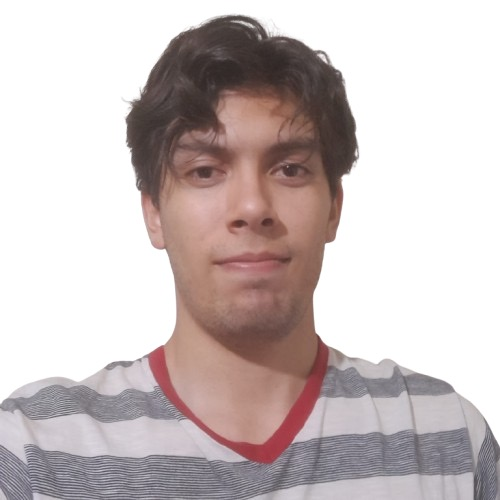
\includegraphics[height=3cm]{Lazaro.jpg} \\
				\textbf{Carranza,}\\ Jesús \\ \texttt{l21330548@hermosillo.tecnm.mx} \\ Teléfono: (6621130410)
			\end{tabular} \\ \vspace{2em}
			\begin{tabular}{c}
				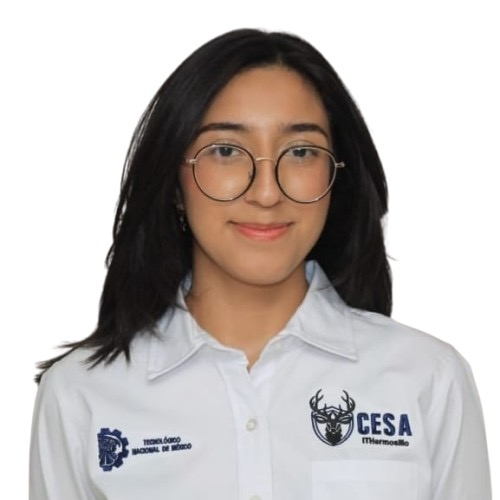
\includegraphics[height=3cm]{Morelia.jpg} \\
				\textbf{Montoya,}\\ Morelia \\ \texttt{l21330642@hermosillo.tecnm.mx} \\ Teléfono: (6624251581)
			\end{tabular} &
			\begin{tabular}{c}
				\includegraphics[height=3cm]{Anitafoto.jpg} \\
				\textbf{Moreno,}\\ Ana \\ \texttt{l21330650@hermosillo.tecnm.mx} \\ Teléfono: (6624591969)
			\end{tabular}
		\end{tabular}
	\end{center}

\end{titlepage}

%	Es innecesario poner el índice porque ya aparece en los marcadores del PDF
%\tableofcontents

% Ejemplo de inclusión de una sección (por ejemplo, "introduccion.tex" debe estar en la carpeta "secciones" y se recomienda no usar carácteres especiales (tilde) o espacios)
\section{Ejercicio 1 - Robot 3}
% TODO: \usepackage{graphicx} required
\begin{figure}[h]
	\centering
	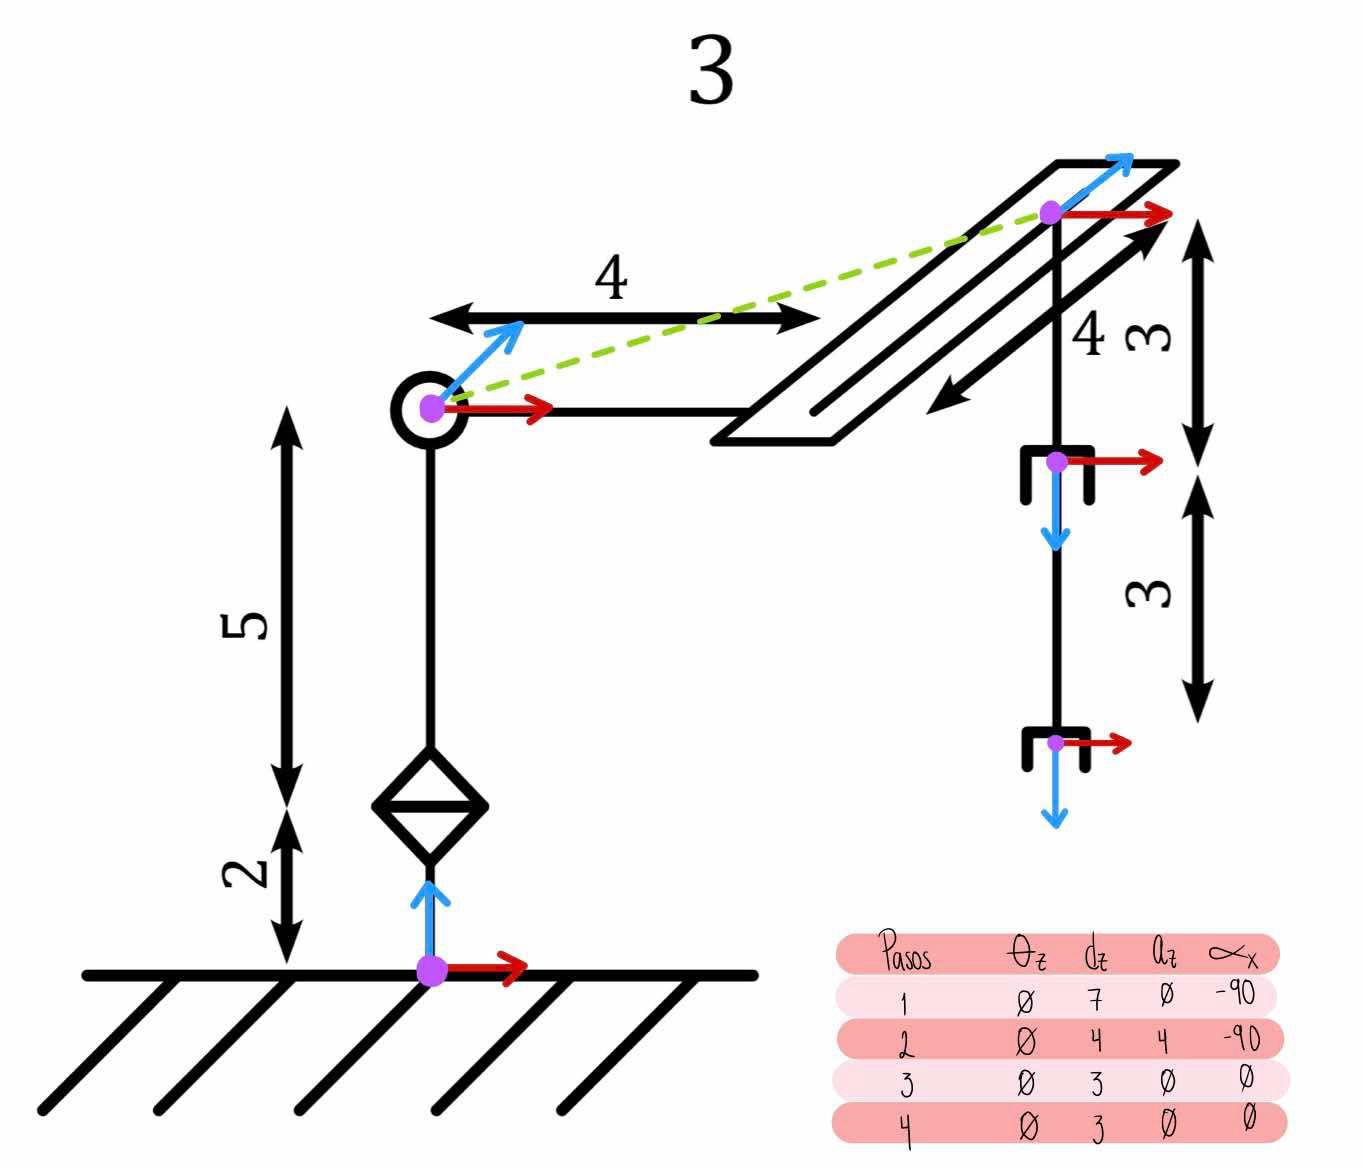
\includegraphics[width=0.63\linewidth]{../img/ejercicio_3-dibujo}
	\caption{Diagráma}
	\label{fig:ejercicio3-dibujo}
\end{figure}
% TODO: \usepackage{graphicx} required
\begin{figure}[h]
	\centering
	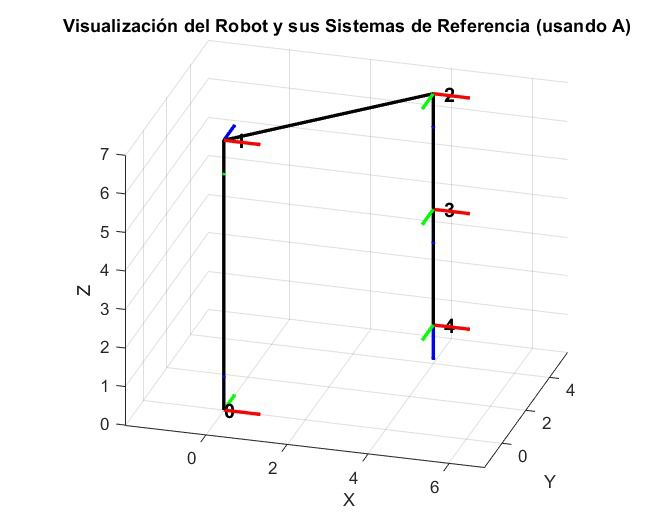
\includegraphics[width=0.66\linewidth]{../img/ejercicio_3-matlab}
	\caption{MATLAB}
	\label{fig:ejercicio3-matlab}
\end{figure}

\newpage
\section{Ejercicio 2 - Robot 4}
\begin{figure}[h]
	\centering
	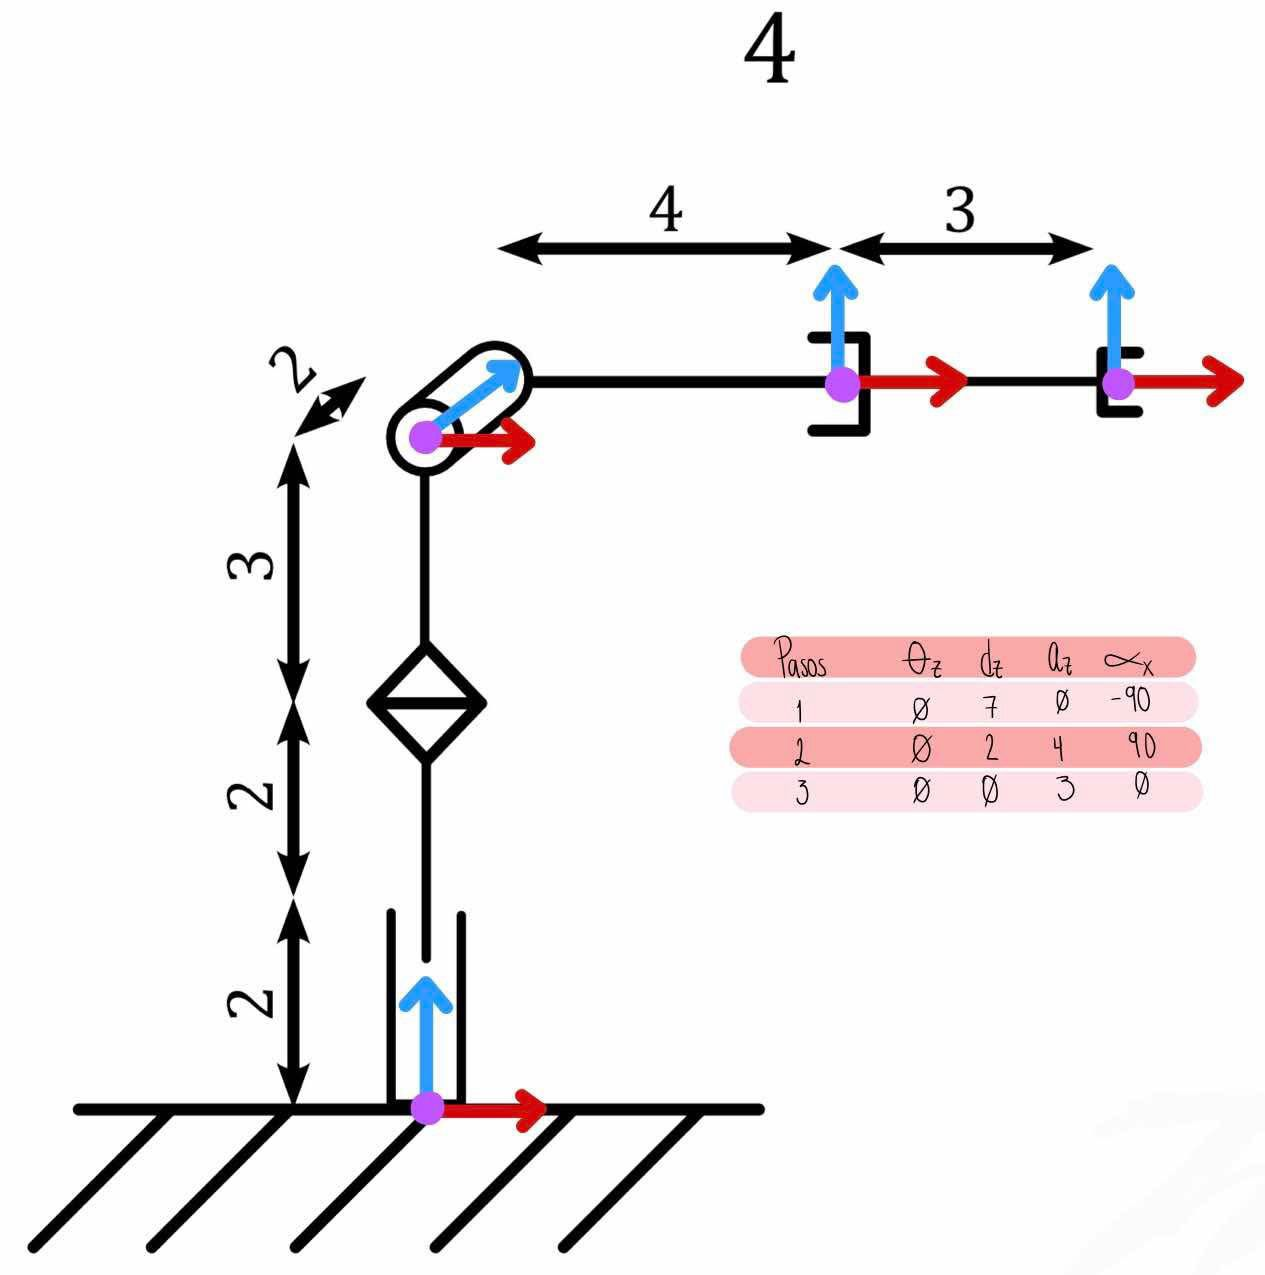
\includegraphics[width=0.58\linewidth]{../img/ejercicio_4-dibujo}
	\caption{Diagráma}
	\label{fig:ejercicio4-dibujo}
\end{figure}

% TODO: \usepackage{graphicx} required
\begin{figure}[h]
	\centering
	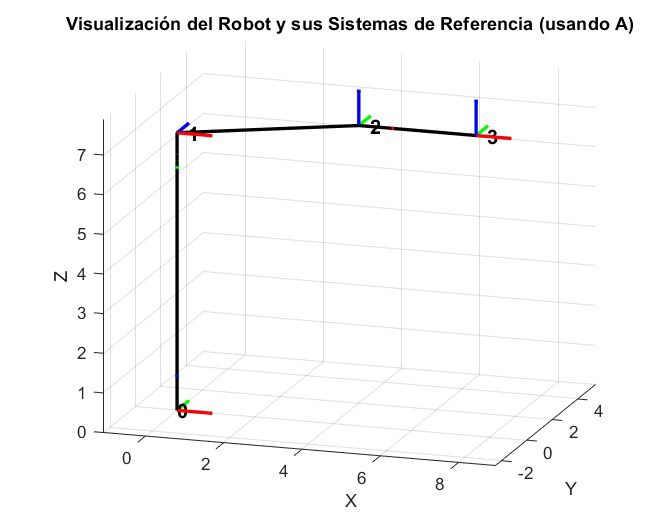
\includegraphics[width=0.58\linewidth]{../img/ejercicio_4-matlab}
	\caption{MATLAB}
	\label{fig:ejercicio4-matlab}
\end{figure}
% TODO: \usepackage{graphicx} required
\newpage
\section{Ejercicio 3 - Robot 5}
\begin{figure}[h]
	\centering
	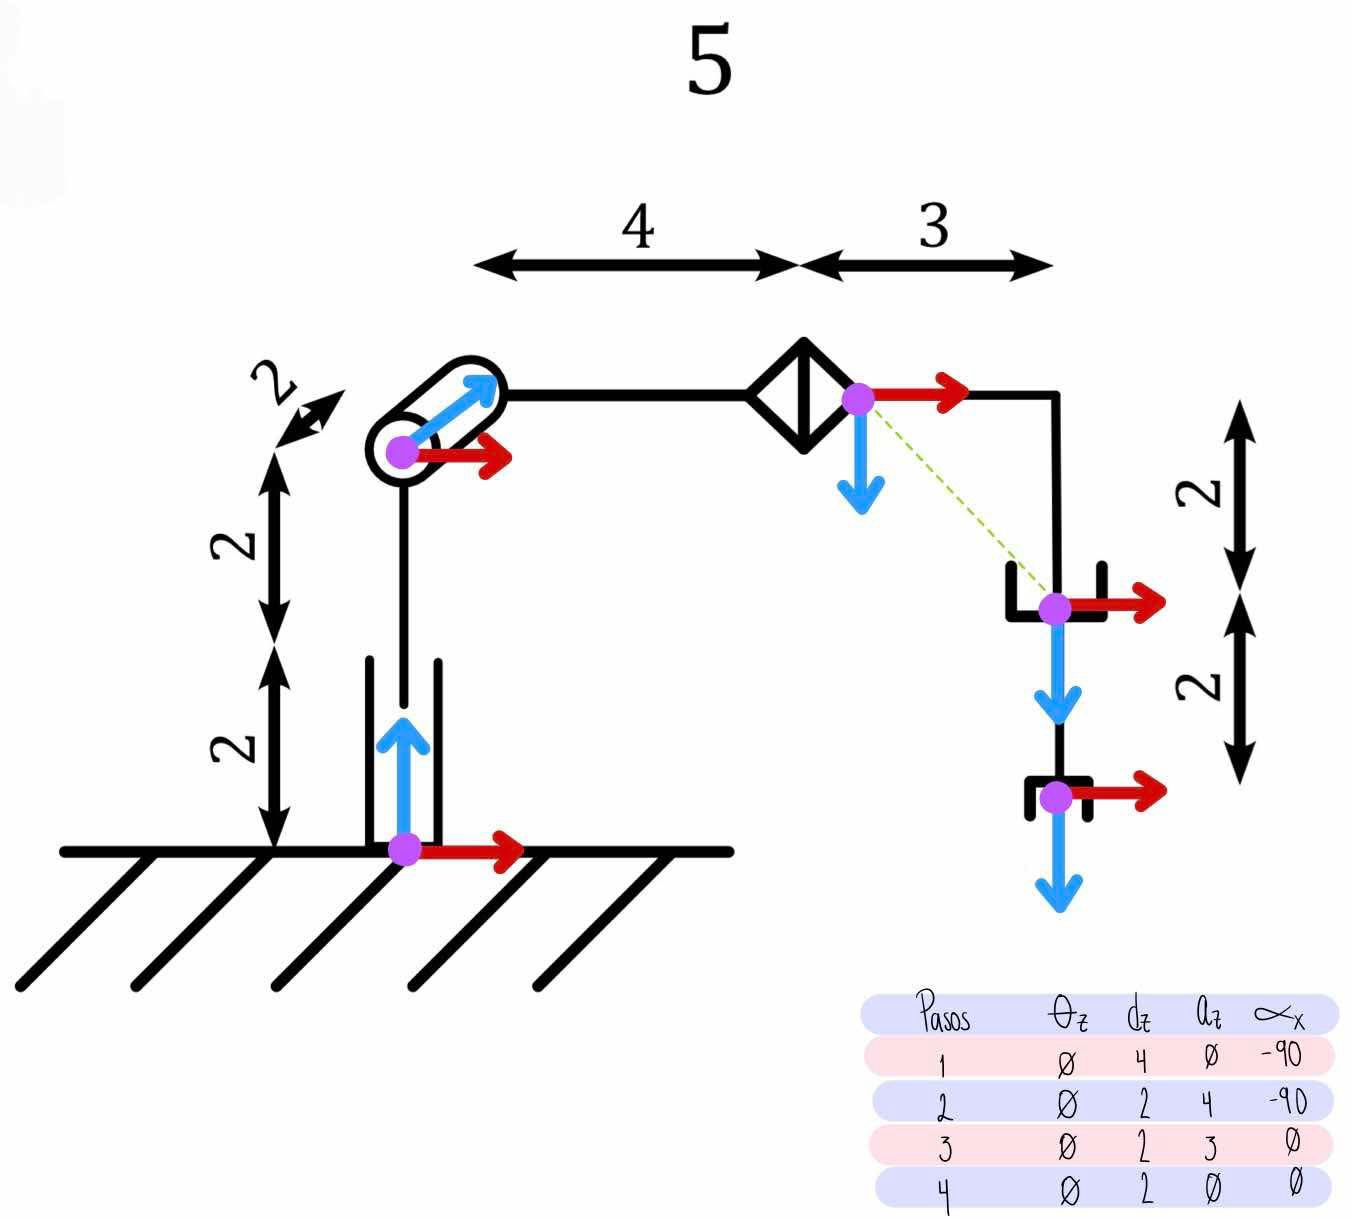
\includegraphics[width=0.6\linewidth]{../img/ejercicio_5-dibujo}
	\caption[Diagráma]{}
	\label{fig:ejercicio5-dibujo}
\end{figure}
\begin{figure}[h]
	\centering
	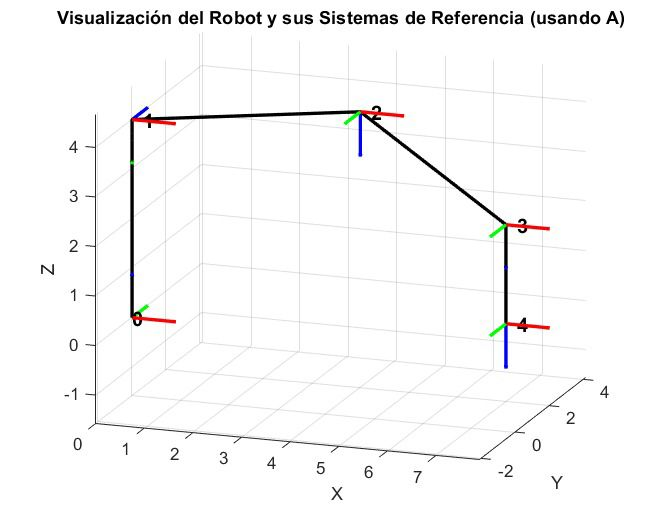
\includegraphics[width=0.6\linewidth]{../img/ejercicio_5-matlab}
	\caption[MATLAB]{}
	\label{fig:ejercicio5-matlab}
\end{figure}

\newpage
\section{Ejercicio 4 - Robot 7}

\begin{figure}[h]
	\centering
	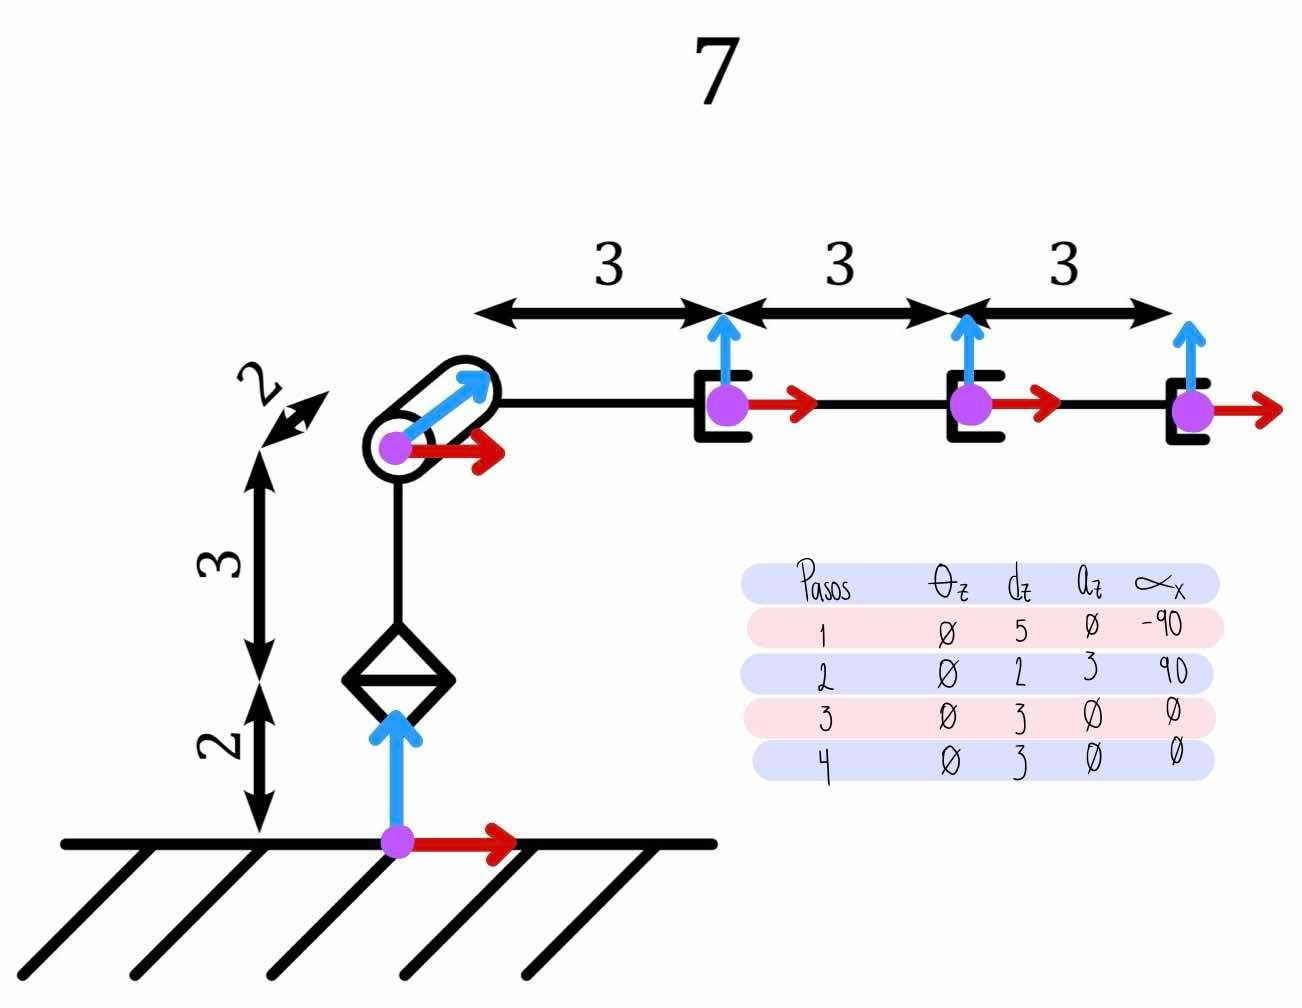
\includegraphics[width=0.6\linewidth]{../img/ejercicio_7-dibujo}
	\caption{Diagráma}
	\label{fig:ejercicio7-dibujo}
\end{figure}

\begin{figure}[h]
	\centering
	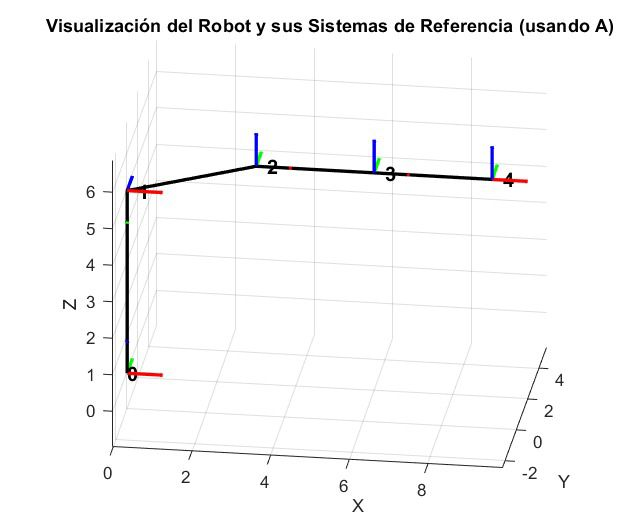
\includegraphics[width=0.6\linewidth]{../img/ejercicio_7-matlab}
	\caption{ MATLAB}
	\label{fig:ejercicio7-matlab}
\end{figure}

\newpage
\section{Ejercicio 5 - Robot 10}
\begin{figure}[h]
	\centering
	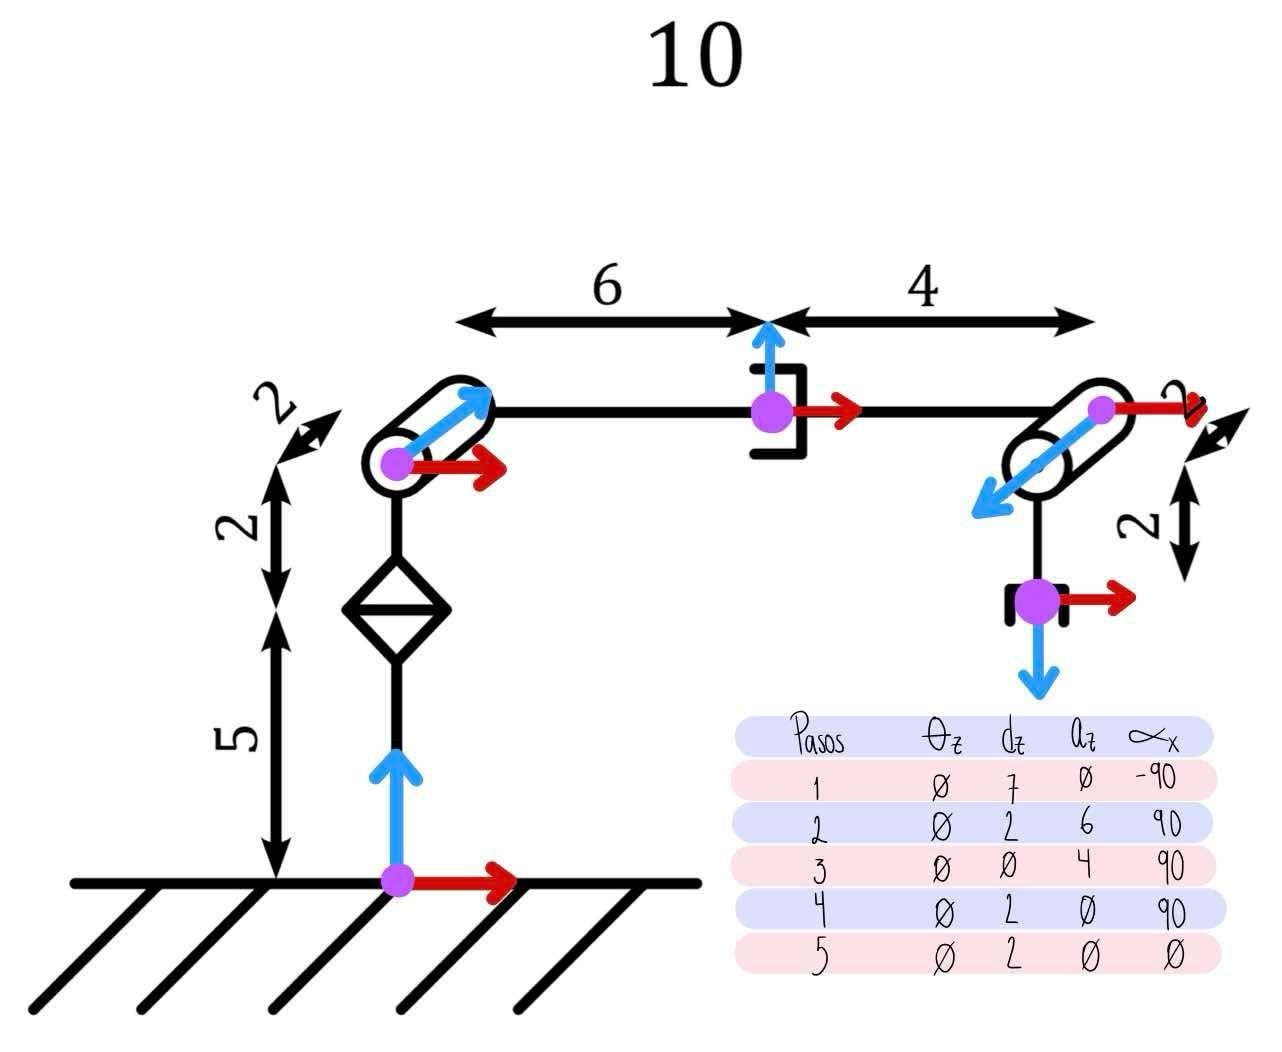
\includegraphics[width=0.55\linewidth]{img/ejercicio_10-dibujo}
	\caption{Digráma}
	\label{fig:ejercicio10-dibujo}
\end{figure}

\begin{figure}[h]
	\centering
	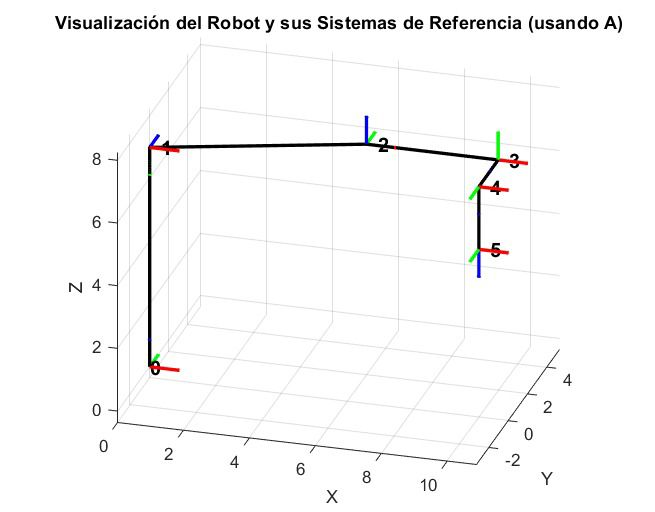
\includegraphics[width=0.55\linewidth]{img/ejercicio_10-matlab}
	\caption{MATLAB}
	\label{fig:ejercicio10-matlab}
\end{figure}


%-------------------------------------------
% Bibliografía
%-------------------------------------------
\bibliographystyle{IEEEtran}  % Estilo de bibliografía IEEE
% La bibliografía se tomará del archivo "fuentes.bib"
%\bibliography{fuentes}
	
\end{document}
